\paragraph{}En esta página se le muestra al usuario el listado de los microcontroladores existentes en el catálogo electronico que satisfacen los parámetros de la búsqueda que él mismo ha realizado, en base a cualquiera de las características de un microcontrolador. Desde dicho listado el usuario podrá añadir al carrito de la compra los microcontroladores que desee pulsando sobre el botón a la derecha de las especificaciones de cada microcontrolador.

\begin{figure}[h!]
	\centering
	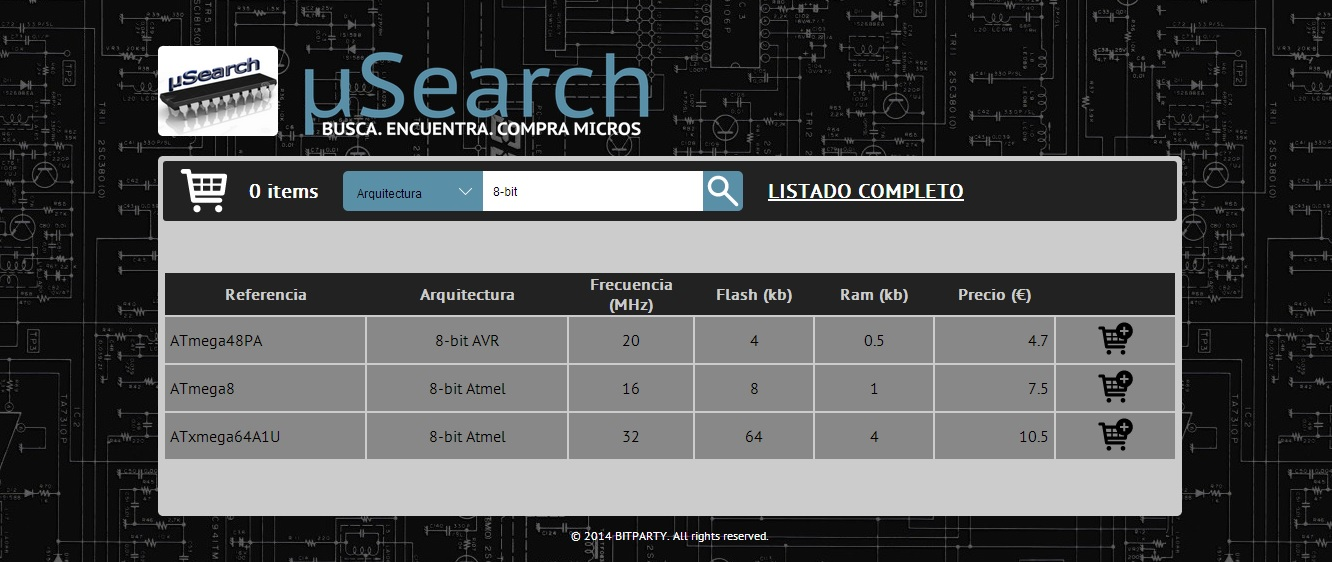
\includegraphics[width=0.85\textwidth]{img/listado_busqueda_user}
	\caption{Página de listado de resultado de búsqueda.}
	\label{fig:listado_busqueda_user}
\end{figure}

Como en todas las demás páginas del sitio web, si se pulsa en cualquiera de los dos logotipos del catálogo $\mu$Search (esquina superior izquierda), el sistema redirigirá al usuario a la página inicial del catálogo.

\paragraph{}Desde esta página, a través de los iconos situados en la cabecera debajo de los logotipos de la web, el usuario puede acceder a:

\begin{itemize}
	\item\textbf{Carrito de la compra:} Pulsando sobre este botón el usuario será redirigido a la página del carrito de la compra.
	
	\item \textbf{Búsqueda:} Desde esta sección de la cabecera, el usuario puede realizar de nuevo una búsqueda distinta sobre el catálogo de microcontroladores en base a cualquiera de las diferentes características de un microcontrolador (Arquitectura, Frecuencia, Flash, RAM). Simplemente se debe seleccionar una de las características de la lista despegable, introducir el texto a buscar y pulsar sobre el icono de búsqueda.
	El usuario será redirigido a una página donde se le mostrará el resultado de la búsqueda en forma de lista de microcontroladores.
		
	\item \textbf{Listado Completo:} Pulsando sobre este botón/icono el usuario será redirigido a la página con el listado completo de microcontroladores del catálogo electrónico.
\end{itemize}